\documentclass[12pt,]{article}
\usepackage{lmodern}
\usepackage{amssymb,amsmath}
\usepackage{ifxetex,ifluatex}
\usepackage{fixltx2e} % provides \textsubscript
\ifnum 0\ifxetex 1\fi\ifluatex 1\fi=0 % if pdftex
  \usepackage[T1]{fontenc}
  \usepackage[utf8]{inputenc}
\else % if luatex or xelatex
  \ifxetex
    \usepackage{mathspec}
  \else
    \usepackage{fontspec}
  \fi
  \defaultfontfeatures{Ligatures=TeX,Scale=MatchLowercase}
\fi
% use upquote if available, for straight quotes in verbatim environments
\IfFileExists{upquote.sty}{\usepackage{upquote}}{}
% use microtype if available
\IfFileExists{microtype.sty}{%
\usepackage{microtype}
\UseMicrotypeSet[protrusion]{basicmath} % disable protrusion for tt fonts
}{}
\usepackage[margin=1in]{geometry}
\usepackage{hyperref}
\hypersetup{unicode=true,
            pdftitle={Do researchers preferentially collaborate with same-gendered colleagues?},
            pdfauthor={Luke Holman* and Claire Morandin; *},
            pdfborder={0 0 0},
            breaklinks=true}
\urlstyle{same}  % don't use monospace font for urls
\usepackage{graphicx,grffile}
\makeatletter
\def\maxwidth{\ifdim\Gin@nat@width>\linewidth\linewidth\else\Gin@nat@width\fi}
\def\maxheight{\ifdim\Gin@nat@height>\textheight\textheight\else\Gin@nat@height\fi}
\makeatother
% Scale images if necessary, so that they will not overflow the page
% margins by default, and it is still possible to overwrite the defaults
% using explicit options in \includegraphics[width, height, ...]{}
\setkeys{Gin}{width=\maxwidth,height=\maxheight,keepaspectratio}
\IfFileExists{parskip.sty}{%
\usepackage{parskip}
}{% else
\setlength{\parindent}{0pt}
\setlength{\parskip}{6pt plus 2pt minus 1pt}
}
\setlength{\emergencystretch}{3em}  % prevent overfull lines
\providecommand{\tightlist}{%
  \setlength{\itemsep}{0pt}\setlength{\parskip}{0pt}}
\setcounter{secnumdepth}{0}
% Redefines (sub)paragraphs to behave more like sections
\ifx\paragraph\undefined\else
\let\oldparagraph\paragraph
\renewcommand{\paragraph}[1]{\oldparagraph{#1}\mbox{}}
\fi
\ifx\subparagraph\undefined\else
\let\oldsubparagraph\subparagraph
\renewcommand{\subparagraph}[1]{\oldsubparagraph{#1}\mbox{}}
\fi

%%% Use protect on footnotes to avoid problems with footnotes in titles
\let\rmarkdownfootnote\footnote%
\def\footnote{\protect\rmarkdownfootnote}

%%% Change title format to be more compact
\usepackage{titling}

% Create subtitle command for use in maketitle
\newcommand{\subtitle}[1]{
  \posttitle{
    \begin{center}\large#1\end{center}
    }
}

\setlength{\droptitle}{-2em}
  \title{Do researchers preferentially collaborate with same-gendered colleagues?}
  \pretitle{\vspace{\droptitle}\centering\huge}
  \posttitle{\par}
  \author{Luke Holman* and Claire Morandin \\ *\textit{luke.holman@unimelb.edu.au} \vspace{5mm}}
  \preauthor{\centering\large\emph}
  \postauthor{\par}
  \date{}
  \predate{}\postdate{}

\usepackage[all]{hypcap} \usepackage{amsmath} \usepackage{booktabs}
\usepackage{caption} \usepackage[labelfont=bf]{caption}
\usepackage{titling} \pretitle{\begin{flushleft}\LARGE}
\posttitle{\par\end{flushleft}\vskip 0.5em}
\preauthor{\begin{flushleft}\large \lineskip 0.5em}
\postauthor{\par\end{flushleft}} \predate{\begin{flushleft}\large}
\postdate{\par\end{flushleft}} \usepackage{fancyhdr} \pagestyle{fancy}
\fancyhead[LO,LE]{\textsl{\leftmark}} \rhead[]{Conference gender ratios}
\usepackage[noabbrev,capitalise]{cleveref} \usepackage{titlefoot}
\usepackage{amssymb} \usepackage{rotating}

\begin{document}
\maketitle
\begin{abstract}
Evidence suggests that women in academia are hindered by conscious and
unconscious biases, and that many female researchers feel excluded from
formal and informal opportunities for research collaboration. In
addition to ensuring fairness and helping redress gender imbalance in
the academic workforce, increasing women???s access to collaboration
could help scientific progress by drawing on more of the available human
capital. Here, we test whether researchers preferentially collaborate
with same-gendered colleagues, using more stringent methods and a larger
dataset than in past work. Our results reaffirm that researchers
co-publish with colleagues of the same gender, and show that this
???gender homophily??? is slightly stronger today than it was 10 years
ago. Contrary to our expectations, we found no evidence that homophily
is driven mostly by senior academics, and no evidence that homophily is
strongest in fields where women are in the minority. Interestingly,
homophily was negatively correlated with journal impact factor
(standardised by research discipline), as predicted if mixed-gender
teams produce better research. \vspace{5mm}
\par\noindent \textbf{Keywords:} Gender bias, Homophily, Scientific
collaboration, Text mining, Women in STEM.
\end{abstract}

\maketitle

\unmarkedfntext{*School of BioSciences, The University of Melbourne, Victoria, Australia}
\newpage

\section{Introduction}\label{introduction}

Women are substantially underrepresented in many branches of the
workforce in science, technology, engineering, mathematics, and medicine
(STEMM), and they face additional challenges and inequities relative to
men (e.g. Larivière et al. 2013; West et al. 2013; Elsevier Report 2017;
Holman et al. 2018). On average, women occupy more junior positions
(Wutte 2007, Reuben, Sapienza \& Zingales, 2014) with lower salaries
(Trower and Chait 2002, Umback 2007), receive less grant money (Hosek et
al. 2005, OER 2005), are promoted more slowly (Hopkins et al. 2013; Long
et al. 1993, Rosenfeld 1991, Zuckerman 1987), and are allocated fewer
resources (European Commission 2009) and less research funding (Feldt
1986, Stack 2004, Larivi??re et al. 2011) than men. Experimental studies
have demonstrated that researchers regard women's achievements less
favourably than identical achievements by men (Moss et al. 2012;
Knobloch et al. 2013).

Because publishing, networking and collaboration are all instrumental to
academic career advancement (Lee and Boheman 2005, Hopkins et al. 2012),
numerous studies have tested for gender differences in these areas
(reviewed in Table S1 in Holman et al. 2018; see also XXX). For example,
studies have shown that relative to men, women tend to be less involved
in international collaboration (Lemoine 1995; Lewison 2001; Webster
2001; Larivi??re et al. 2011, Bozeman and Corley 2004), collaborate less
with researchers from their own university department (Websters 2001),
have less prestigious collaborations (Long 1990), and fewer
collaborations in general (Fuchs Von Stebut and Allmendinger 2001).
Possible explanations for the smaller average professional networks of
women include a greater average amount of family obligations (Long 1990,
Wright et al. 2003, Reskin 1978), lower participation of women in
international conferences (Lewison 2001, Eisen 2014, Martin 2014), and
reduced receipt of research travel funds by women (Bozeman and Corley
2004).

A high, steadily increasing proportion of research papers is written by
more than one author (West et al. 2013), making collaboration a key
predictor of publication output, and in turn, a key predictor of career
prospects (Cohn et al 2014, Jordan et al. 2008, Tower et al. 2007).
Additionally, empirical studies suggest that mixed-gender (Campbell et
al. 2013) or otherwise diverse (Hong and Page 2004) teams can produce
better results on collaborative tasks. For reasons such as these,
several studies have tested for gender differences in collaboration
frequency or pattern by examining the author lists of published
research. To our knowledge, every study of this question has concluded
that men publish with other men, and women with women, more often than
expected if collaborators assort randomly with regards to gender (Ferber
and Teiman, 1980; McDowell and Smith 1992; Ghiasi et al. 2015; Crow and
Smykla 2015, Zettler et al. 2016, Fahmy and Young, 2016, Jadidi et al.
2017; Teele and Thelen 2017, Araujo and Fontainha 2017a,b). This
preference for same-gendered colleagues is often termed ???gender
homophily???.

However, we hypothesise that these studies of gender homophily were
hindered by a sampling issue that we term the Wahlund effect
(\autoref{wahlund_plot}), making the true extent of homophily difficult
to ascertain from present data. Essentially, whenever samples are taken
from two or more discrete sets of literature, which vary in the author
gender ratio and which are largely not connected by collaboration, the
number of same-gendered coauthors will be inflated. This can make it
appear as though authors preferentially publish with same-gendered
colleagues if no gender preferences exist, or even if researchers
preferentially select opposite-gendered colleagues. For example, a
sample of bioinformatics and cell biology papers might contain an excess
of mostly-male and mostly-female author lists, simply because
researchers preferentially work with colleagues from the same
discipline, and because more women work in cell biology than in
bioinformatics (Holman et al. 2018). We name this issue after the
Wahlund effect in population genetics (Wahlund 1928), whereby spatial
differences in allele frequencies create an excess of homozygotes across
the whole population, even if alleles assort randomly within each
subpopulation.

In the present study, we test whether academics tend to co-publish with
same-gendered collaborators, while controlling for the Wahlund effect as
strictly as possible. Our study uses a recently-published dataset
describing the gender of 35.5m authors from 9.15m articles indexed on
PubMed (Holman et al. 2018). Holman et al. (2018) reported large
differences in the gender ratio of authors across research disciplines,
journals, countries, and across the years 2002-2016. We therefore tested
for gender homophily after restricting the analysis to particular
journals (i.e.~research specialties), time periods, and countries.

\section{Methods}\label{methods}

\subsection{Obtaining author lists and assigning
gender}\label{obtaining-author-lists-and-assigning-gender}

We used the dataset of PubMed author lists from Holman et al. (2018).
Briefly, that dataset was created by downloading every single article
indexed on PubMed, from the oldest articles up to the present (which was
August 2016), and attempting to assign a gender to each author based on
their given name, using the web service genderize.io. Each journal was
assigned to one of 107 scientific disciplines (e.g. ???Nephrology??? or
???Cell Biology???), using PubMed???s journal categorisations where
available. Because the present study focuses on co-authorship, all
single-author papers were removed from the dataset. To simplify the
statistical analysis, we also discarded all papers for which we could
not determine the gender of every author with at least 95\% certainty.
To mitigate Wahlund effects caused by variation in the gender ratio of
researchers over time (see below), we also discarded all papers except
those that were published 0-1 or 10-11 years before the PubMed data were
collected (i.e.~20 August 2016). Lastly, we excluded journals with fewer
than 50 suitable papers. This left us with a dataset from August 2015 -
August 2016 containing 276,879 papers with 1,311,213 authorships, and a
dataset from August 2005 - August 2006 containing 151,652 papers and
647,634 authorships. These papers came from 2,116 and 1,192 journals
respectively, which were grouped into 107 and 101 research disciplines.
There was a median of 87 (87) papers per journal, 413 (371) authors per
journal, and 4 (4) authors per paper (the first number is for 2015-6,
and the bracketed number for 2005-6).

\subsection{\texorpdfstring{Calculating \(\alpha\), the coefficient of
homophily}{Calculating \textbackslash{}alpha, the coefficient of homophily}}\label{calculating-alpha-the-coefficient-of-homophily}

Inspired by Bergstrom et al.
(\url{http://www.eigenfactor.org/gender/assortativity/measuring_homophily.pdf}),
we defined the coefficient of homophily as \(\alpha = p - q\), where
\(p\) is the probability that a randomly-chosen co-author of a
\emph{male} author is a man and \(q\) is the probability that a
randomly-chosen co-author of a \emph{female} author is a man. Therefore,
\(\alpha\) \textgreater{} 0 suggests that same-gender authors publish
together more often than expected if authors assort randomly with
respect to gender (homophily), \(\alpha\) \textless{} 0 suggests that
opposite-gender authors publish together more often than expected
(heterophily), and \(\alpha\) = 0 suggests random assortment with
respect to gender.

To estimate \(\alpha\) for a particular subset of the scientific
literature, we estimated \(p\) as the average proportion of men???s
co-authors who are men (averaged across all papers with at least one man
author), and \(q\) as the average proportion of women???s co-authors who
are men (averaged across all papers with at least one woman author). To
estimate the 95\% confidence intervals on \(\alpha\) for a given set of
\(n\) papers, we sampled \(n\) papers with replacement 1000 times,
estimated \(\alpha\) on each sample, and recorded the 95\% quantiles of
the 1000 resulting estimates.

As well as calculating \(\alpha\) for all authors, we calculated
\(\alpha\) for first and last authors only. \(\alpha\) was again defined
as \(p - q\), but this time \(p\) was estimated as the average
proportion of male co-authors on papers with a male first/last author,
and \(q\) was estimated as the average proportion of male co-authors on
papers with female first/last authors. We did not calculate \(\alpha\)
for other authorship positions (e.g.~second or third authors) because
this would necessitate reducing the dataset to papers with a
sufficiently long authorship list, complicating comparison with other
authorship positions that were calculated using a different sample.

Our test assumes that the expected value of \(\alpha\) is zero if
authors randomly assort, but for small datasets this assumption is not
always true (as pointed out by Carl T. Bergstrom in a blog post,
\url{http://www.eigenfactor.org/gender/assortativity/note_to_eisen.rtf}).
To borrow Prof.~Bergstrom???s example, consider a small research
specialty comprising just two men and two women researchers, who have
together produced six two-author papers: one paper in each of the six
possible two-author combinations. For these six papers, \(\alpha\) =
\(-\frac{1}{3}\), even though same- and opposite-gendered coauthors were
selected in equal proportion to their frequency in the pool of possible
collaborators. To control for the fact that the null expectation for
\(\alpha\) is not necessarily zero (particularly for very small
datasets), we devised an adjusted version of the coefficient of
homophily, which we term \(\alpha'\). Every time we calculated
\(\alpha\) for a set of papers, we also determined the expected value of
\(\alpha\) under the null hypothesis that authors assort randomly with
respect to gender. This was accomplished by randomly shuffling authors
across papers 1000 times, recalculating \(\alpha\), and taking the
median. We then calculated \(\alpha'\) by subtracting the null
expectation for \(\alpha\) from the observed value. We also used the
null-simulated \(\alpha\) values to calculate a two-tailed p-value for
the observed value of \(\alpha\); the p-value was defined as the
proportion of null simulations for which
\(|\alpha_{null}| > |\alpha_{obs}|\). We applied false discovery rate
correction to each set of p-values to account for multiple testing
(Benjamini and Hochberg 1995).

As expected, \(\alpha'\) was usually almost identical to \(\alpha\)
(Figure S1), but \(\alpha\) was downwardly biased relative to
\(\alpha'\) for small datasets (Figure S2). Additionally, the
correlation between \(\alpha'\) and sample size was negligible (\(R^2\)
\textless{} 0.01), suggesting that \(\alpha'\) effectively removed the
dependence of \(\alpha\) on sample size. We therefore used the adjusted
statistic \(\alpha'\) in all our analyses.

\subsection{Minimising the Wahlund effect: discipline and time
period}\label{minimising-the-wahlund-effect-discipline-and-time-period}

As discussed in the Introduction, the Wahlund effect can give the
appearance of gender homophily (reflected in our study as \(\alpha'\)
\textgreater{} 0) whenever one lumps together different
???subpopulations??? of academic papers that differ in their author
gender ratios (Figure 1).

To minimise bias in \(\alpha'\) due to the Wahlund effect, we restricted
each set of papers to a single research specialty to the greatest extent
allowed by our data. Specifically, we only calculated \(\alpha'\) for
individual journals, since papers from the same journal typically focus
on one or a few closely related topics. Although some journals, e.g.
\emph{PLoS ONE}, publish research from diverse disciplines with very
different author gender ratios (Holman et al. 2018), calculating
\(\alpha'\) for these highly multidisciplinary journals is still useful
as a contrast. The difference in \(\alpha'\) between highly
multidisciplinary and more specialised journals, e.g. \emph{PLoS ONE}
versus \emph{PLoS Computational Biology}, gives a rough estimate of the
extent to which multidisciplinarity can inflate \(\alpha'\).

As well as varying between disciplines, the gender ratio of authors has
changed markedly over time (Holman et al. 2018). Because the gender
ratio was more male-biased in the past, \(\alpha'\) would be inflated if
we calculated it for a sample of papers published over a long time
frame. To minimise this effect, we only sampled papers from two one-year
periods (namely 2005-6 and 2015-16). The median change per year in \%
(fe)male authors across journals is \textless{} 0.5\% (Holman et al.
2018), and so restricting our dataset to a single year should prevent
temporal changes in gender ratio from noticeably inflating our estimates
of \(\alpha'\).

\subsection{Minimising the Wahlund effect: author country of
affiliation}\label{minimising-the-wahlund-effect-author-country-of-affiliation}

A Wahlund effect could arise even if one calculates \(\alpha'\) for a
single discipline and time period, because of variation in the gender
ratio of researchers from different countries. For example, Holman et
al. (2018) showed that authors based in Serbia are more than twice as
likely to be women as are authors based in Japan. Therefore, a dataset
containing a mix of papers from teams of authors based in these two
countries would probably contain an excess of same-sex coauthorships,
even if collaboration were random with respect to gender within each
country.

To address this, we also analysed every combination of journal and
author country of affiliation for which we had enough data (i.e.~50 or
more papers published in 2015-16). For simplicity, we restricted the
dataset to only include papers for which Holman et al. (2018) had
identified the country of affiliation for all authors on the paper, and
all authors shared the same country of affiliation. Restricting the
dataset in this fashion produced enough data to measure \(\alpha'\) for
325 combinations of journal and country (median: 70 papers and 273
authors per combination).

\subsection{Calculating standardised journal impact
factor}\label{calculating-standardised-journal-impact-factor}

We obtained the 3-year impact factor for each journal from Clarivate
Analytics. To account for large differences in impact factor between
disciplines, we took the the residuals from a model with \(Log_{10}\)
impact factor as the response and the research discipline of the journal
as a random effect. Thus, journals with a positive standardised impact
factor have a higher mean number of citations than the average for
journals in their discipline. We then used Spearman rank correlation to
test whether our estimates of gender homophily covaried with journal
impact factor.

\subsection{Statistical analysis}\label{statistical-analysis}

Previous authors (e.g.~Bonham \& Stefan 2017) have hypothesised that
senior scientists preferentially recruit staff and students of the same
gender, and/or that junior researchers preferentially select
same-gendered mentors. In the majority of disciplines, authorship
conventions mean that the first-listed author is often an early-career
researcher, while the author listed last is more likely to be a senior
researcher leading a research team (Wren et al. 2007). Assuming that
senior researchers are the main drivers of homophily and that there are
enough papers with three or more authors, we predict that the last
author???s gender will be the strongest predictor of the remaining
authors??? genders (i.e.~the gender of the last author will be more
salient than that of the first author, or any other authorship
position). This is because the first author???s gender would simply be
an imperfect correlate of the true causal effect, while the last
author???s gender would be the causal effect itself.

To test whether \(\alpha'\) for last authors tends to be higher than
\(\alpha'\) for first authors for any given dataset, we used a linear
mixed model implemented in the \texttt{lme4} and \texttt{lmerTest}
packages for R, with \emph{authorship position} (first or last) as a
fixed factor, and \emph{journal} and \emph{research discipline} as
crossed random effects. The response variable was \(\alpha'\), and we
weighted each observation by the inverse of the standard error from our
estimate of \(\alpha'\), meaning that more accurate measurements of
\(\alpha'\) had more influence on the results. We used a similar model
to test for a difference in \(\alpha'\) between the 2005-6 and the
2015-16 datasets, with two differences: instead of authorship position,
we fit year range as a two-level fixed factor, and used \(\alpha'\)
estimated for all authors (not first/last authors) as the response
variable.

The relationship between the gender ratio of authors publishing in a
journal and its \(\alpha'\) value appeared nonlinear (Figure 4). We
therefore fit a generalised additive model with thin plate regression
spline smoothing, implemented using the \texttt{mgcv} package for R.

\section{Results}\label{results}

\subsection{Gender homophily by discipline, time period, and authorship
position}\label{gender-homophily-by-discipline-time-period-and-authorship-position}

\autoref{alpha_histograms} shows the distribution of \(\alpha'\)
estimates in 2015-2016 across all journals for which we recovered
sufficient data, when \(\alpha'\) was calculated for all authors, first
authors only, or last authors only. The great majority of journals had
\(\alpha'\) \textgreater{} 0, and for many of these the corrected
two-tailed p-values suggested that \(\alpha'\) was significantly greater
than zero (1469/2077 journals were significant in 2015-16, and 404/1192
in 2005-6). Only 2/2077 journals had statistically significantly
heterophily (i.e. \(\alpha'\) \textless{} 0) in 2015-16, and 1/1192 in
2005-6. The remaining 606 or 787 journals (in 2015 and 2005
respectively) had a value of \(\alpha'\) not significantly different
from zero, such that we could not reject the null hypothesis of random
assortment with respect to gender.

\(\alpha'\) was significantly higher in the sample from 2015-16 relative
to 2005-6, but the difference in means was small (Figure S3; Effect of
the fixed factor ???time period??? in a linear mixed model of the data
for all author positions: Cohen???s \(d\) = 0.09??0.04, \(t_{948}\) =
2.51, p = 0.012).

When comparing pairs of \(\alpha'\) values estimated for the first and
last authors for the same journals, we found that \(\alpha'\) tended to
be higher for first authors than for last authors (Figure S4; Effect of
the fixed factor ???Authorship position??? in a linear mixed model:
Cohen???s \(d\) = 0.07??0.02, \(t_{1988}\) = 4.48, p \textless{}
0.0001). This suggests that the gender of the first author was a
slightly stronger predictor of the remaining authors??? genders than the
gender of the last author, i.e.~the opposite of our prediction based on
the hypothesis that senior scientists are causally responsible for
homophily.

\subsection{Possible differences in the strength of homophily between
disciplines}\label{possible-differences-in-the-strength-of-homophily-between-disciplines}

\autoref{alpha_histograms} illustrates the variance in journal homophily
values (\(\alpha'\)) across scientific disciplines. All disciplines had
a positive average \(\alpha'\), although homophily appeared somewhat
stronger in some disciplines than others (e.g.~mean \(\alpha'\) was
0.12??0.02 for Urology journals, and 0.03??0.01 for Veterinary Medicine
journals; \autoref{alpha_histograms}, Table S3). However, there was
little evidence for strong differences in \(\alpha'\) between
disciplines: the random factor ???discipline??? explained at most 1\% of
the variance in \(\alpha'\) in the two linear mixed models described in
the previous section (see \autoref{alpha_histograms} and mixed models in
Online Supplementary Material). This implies that the processes causing
positive \(\alpha'\) are similarly strong in all the disciplines we
examined.

There was no indication that journals publishing on a wide range of
topics have higher \(\alpha'\) values than more specialised journals,
due to the Wahlund effect. For example, the journal category
???Multidisciplinary??? - which includes journals like \emph{PLoS ONE},
\emph{Nature}, \emph{Science}, and \emph{PNAS} - did not have notably
elevated \(\alpha'\) (\autoref{alpha_histograms}). This result suggests
that our estimates of homophily, and estimates from earlier studies, are
not notably inflated by the presence of disparate research topics (with
variable author gender ratios) being published within individual
journals.

\subsection{Relationship between gender homophily and gender
ratio}\label{relationship-between-gender-homophily-and-gender-ratio}

We next tested whether researchers are more or less likely to seek out
same-gendered colleagues in strongly gender-biased disciplines
(e.g.~Surgery or Nursing), relative to disciplines with a comparatively
gender-balanced workforce (e.g.~Psychiatry). We found a positive,
non-linear relationship between the overall gender ratio of all authors
publishing in a particular journal (as estimated by Holman et al. 2018),
and the estimated value of \(\alpha'\) for all authors and for first
authors (\autoref{alpha_gender_ratio}). Journals with a balanced or
female-biased author gender ratio tended to have higher \(\alpha'\) than
journals with a male-biased author gender ratio (GAM smooth terms p
\textless{} 0.001, see Online Supplementary Material). The relationship
was not statistically significant when \(\alpha'\) was calculated for
last authors (GAM, p = 0.142), though the trend appeared similar
(\autoref{alpha_gender_ratio}).

\subsection{Relationship between journal impact factor and gender
homophily}\label{relationship-between-journal-impact-factor-and-gender-homophily}

We observed a noisy but statistically significant linear relationship
between discipline-standardised journal impact factor and \(\alpha'\),
such that journals with a high impact factor for their discipline had
weaker gender homophily than did journals with a low impact factor for
their discipline (\autoref{impact_factor}; linear regression: \(R^2\) =
0.043, \(t_{1415}\) = -8.0, p \textless{} 0.0001).

\subsection{Analysis correcting for differences between
countries}\label{analysis-correcting-for-differences-between-countries}

When we restricted the analysis to only include authors with
affiliations from a single country, we found statistically significant
homophily for 72 of the 325 journal-country combinations tested (64
unique journals and 18 unique countries), and no significant evidence of
heterophily (Figures S5-S6). Additionally, the values of \(\alpha'\)
calculated for each journal-country combination were mostly very similar
to the \(\alpha'\) values calculated for the journal as a whole
(i.e.~when pooling papers from different countries); the average
difference in \(\alpha'\) was 0.002 (Figure S7). These results suggest
that our findings of widespread homophily in the main analysis cannot
solely be driven by a Wahlund effect resulting from gender differences
between countries.

\section{Discussion}\label{discussion}

We found evidence that researchers tend to publish with same-gendered
coauthors, despite implementing stringent controls for ???spurious???
homophily resulting from Wahlund effects (\autoref{wahlund_plot}). Our
data therefore reaffirm earlier conclusions (Ferber and Teiman 1980;
McDowell and Smith 1992; Crow and John Ortiz (2015); Ghiasi et al. 2015;
Zettler et al. 2016; Fahmy and Young 2016; Jadihi et al. 2017; Araujo
and Fontainha 2017a; Teele and Thelen 2017) that research collaborations
occur between same-gendered colleagues substantially more often than
expected if collaborators are selected without regard to their gender.
Many journals had \(\alpha'\) values over 0.1, meaning that the gender
ratio of the average man's coauthors is skewed towards men by
\textgreater{}10\%, relative to the gender ratio of a woman's coauthors.
Few journals had \(\alpha'\) values below zero, and fewer still had
significantly negative \(\alpha'\) values, suggesting that it is
comparatively rare for researchers to preferentially select
opposite-gendered collaborators.

We found no evidence that gender homophily is restricted to particular
disciplines: instead, there was evidence of homophily across many
diverse research disciplines. We also found that gender homophily was
marginally stronger in 2015-2016, relative to 2005-2006. This result
suggests that recent increases in the number of women working in STEMM,
as well as recent efforts to recruit, retain, and celebrate women in
STEMM, have co-occurred with rise in the frequency of same-gender
collaborations, not a fall. We speculate that this trend might result,
at least in part, from the increasing number of women working in senior
positions in STEMM over the last 10 years (DATA?). Because many
co-authorships involve a junior and a senior researcher (e.g.~a student
and professor), and the gender ratio is typically more skewed among
senior staff (Shaw and Stanton ref), there will be more opposite-gender
collaborations than expected if the gender ratio were the same at both
career stages. Thus, the observed increase in homophily might be due to
the greater numbers of women working in leading roles.

Gender homophily was slightly stronger in research disciplines with a
female-biased gender ratio, as compared to male-biased or
gender-balanced fields. One interpretation of this result is that men
are more likely to seek out other men in fields in which men are in the
minority, relative to the homophily shown by women in fields in which
women are in the minority.

We also found that journals with a high impact factor (relative to other
journals in the same research discipline) tended to have weaker gender
homophily than did low-impact journals. If one accepts the contentious
claim that papers published in high-impact journals tend to be of higher
quality than those in low-impact journals (e.g. Garfield 2006), then
this result provides correlational support for the hypothesis that
mixed-gender teams produce better research than single-gender teams
(Campbell et al. 2013).

Contrary to our expectations, we found no evidence that homophily is
driven mostly by senior academics, and no evidence that homophily is
strongest in fields where women are in the minority. Interestingly,
homophily was negatively correlated with journal impact factor
(standardised by research discipline), as predicted if mixed-gender
teams produce better research.

Academic publishing is one of the most (if not the most) important tool
for a researcher to display their work, and is frequently used as a
success indicator for being promoted, hired as a faculty member, or
being invited as plenary speaker. Our finding that researchers are more
likely to publish with same-gendered coauthors implies that
co-authorship listing is not a random process, but instead creates
additional gender imbalance. Homophily could make it harder for women to
find collaborators in disciplines where women are in the minority
(i.e.~almost all STEMM fields; Holman et al. 2018). Because women make
up for as little as 30\% of the STEMM scientist community (REF), they
are therefore less likely to be picked as coauthors, and, as a result,
gender homophily creates further gender imbalance and disadvantages for
women. Men tend to publish more in high impact journals (REF) as first
author, and generate more citations than papers lead by first author
women (REF). As a consequence, gender homophily is also likely to
contribute to lower publication rates for women (McDowell and Smith
1992), and lower scientific success (REF).

Why does gender homophily exists in science? Collaboration often leads
to co-authorship publications, citations and additional professional
recognitions, therefore first author should always be considering
collaborators that are most likely to enhance their productivity and in
the long term also their academic success, rather than pick co-authors
according to their gender. First of all, it is likely that decades ago,
the probability to meet a woman colleague working on the same area of
expertise was slimmer than now. However, the number of women in STEM is
increasing, and it is not likely to be an obstacle to collaboration
nowadays.

\section{Acknowledgements}\label{acknowledgements}

We are grateful to XXXX.

\section{References}\label{references}

\hypertarget{refs}{}
\hypertarget{ref-Crow_2015}{}
Crow, M. S., and S. John Ortiz. 2015. The effect of gender‐sorting on
propensity to coauthor: Implications for academic promotion. American
Journal of Criminal Justice 40:441--455.

\hypertarget{ref-Elsevier_report}{}
Elsevier Report. 2017. Gender in the global research landscape.
elsevier.com/research-intelligence/resource-library/gender-report.

\hypertarget{ref-Garfield_2006}{}
Garfield, E. 2006. The history and meaning of the journal impact factor.
JAMA 295:90--93.

\hypertarget{ref-Holman_2018}{}
Holman, L., D. Stuart Fox, and C. E. Hauser. 2018. The gender gap in
science: How long until women are equally represented? PLoS Biology
16:e2004956.

\hypertarget{ref-Lariviere_2013}{}
Larivière, V., C. Ni, Y. Gingras, B. Cronin, and C. R. Sugimoto. 2013.
Bibliometrics: global gender disparities in science. Nature
504:211--213.

\hypertarget{ref-West_2013}{}
West, J. D., J. Jacquet, M. M. King, S. J. Correll, and C. T. Bergstrom.
2013. The role of gender in scholarly authorship. PLoS ONE 8:e66212.

\newpage

\section{Figures}\label{figures}

\begin{figure}
\centering
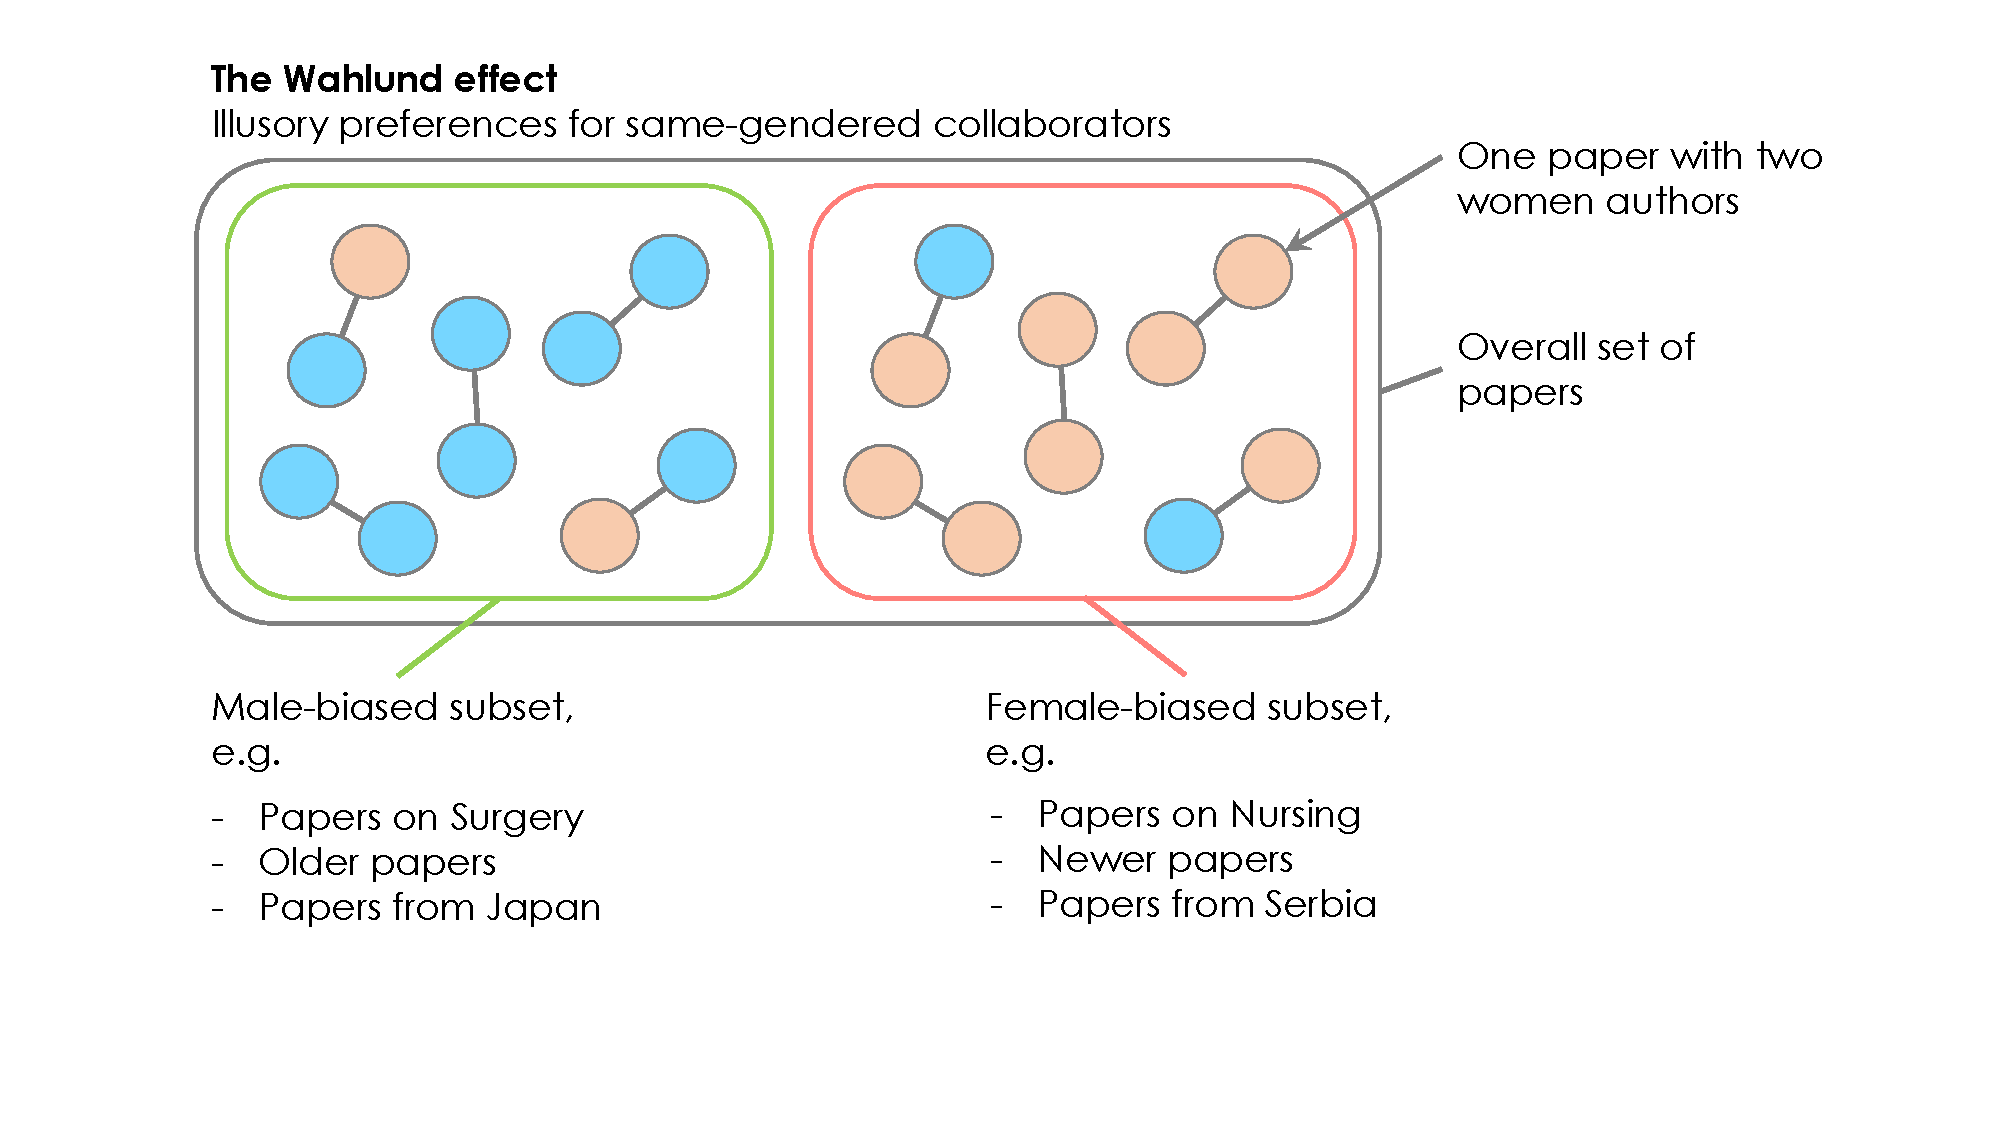
\includegraphics{../figures/Figure 1 - Wahlund figure.pdf}
\caption{The Wahlund effect can make it appear as if authors prefer to
publish with same-gendered colleagues, even if no such preference
exists. Here, coloured circles represent male and female authors, and
coauthors are linked with lines. Across the whole set of ten papers,
there is an apparent excess of same-gender collaborations. Specifically,
there are six same-gender papers and only four mixed-gender papers,
which is fewer than the \(10\times2\times0.5\times0.5 = 5\) mixed-gender
papers we would expect under the null hypothesis that authors assort
randomly with respect to gender. However, within each subset, there is
no evidence that authors prefer to publish with same-gendered
individuals. The Wahlund effect will tend to inflate the frequency of
same-sex coauthors whenever the data is composed of two or more
disconnected subsets of literature with different author gender ratios;
these subsets could be research disciplines, older versus newer papers,
or papers from authors in different countries. \label{wahlund_plot}}
\end{figure}

\newpage

\begin{figure}
\centering
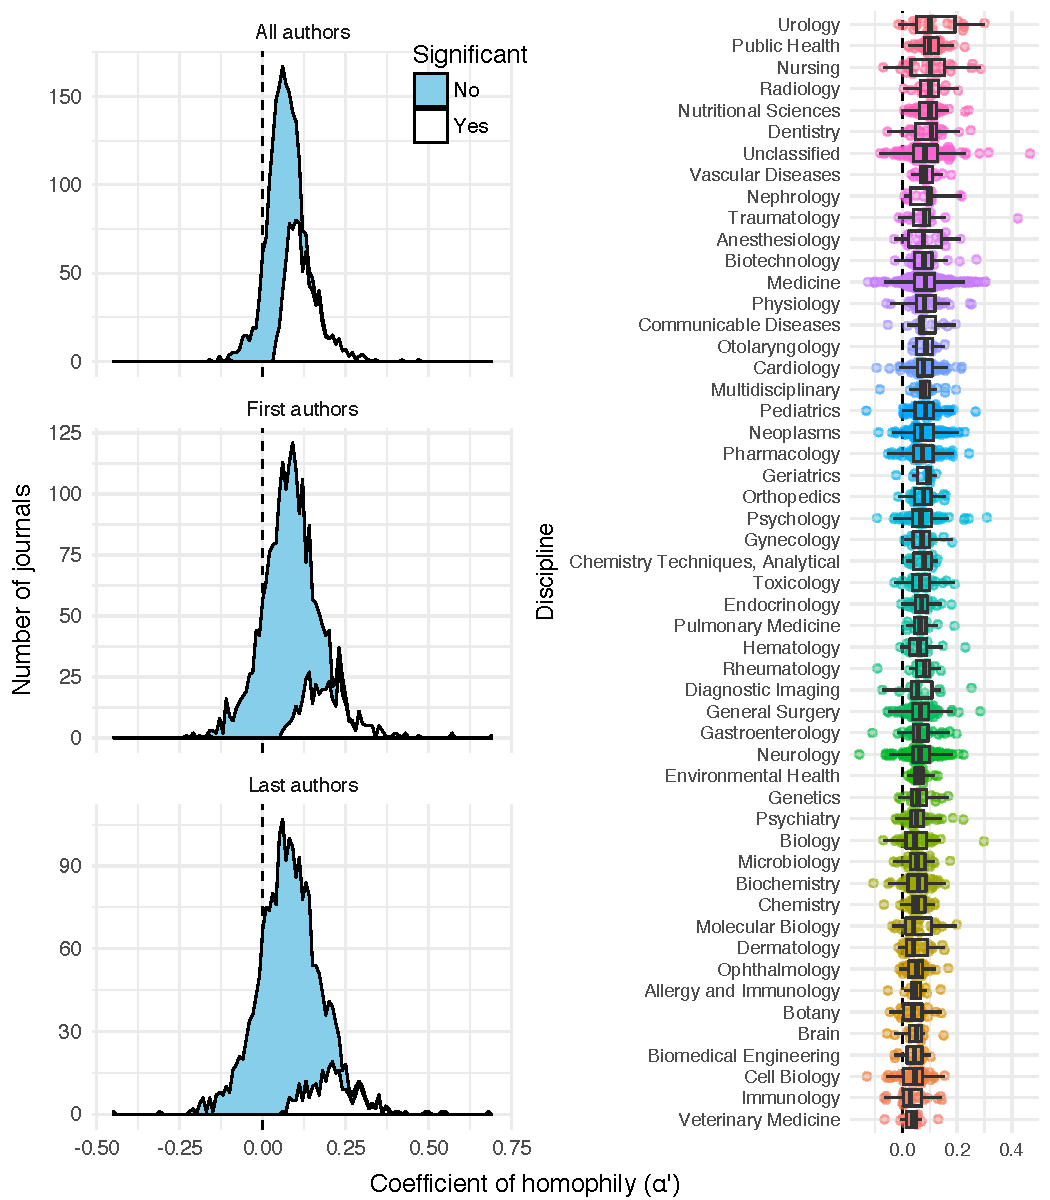
\includegraphics{../figures/figure2.pdf}
\caption{Of the 2077 journals for which we had adequate data in
2015-2016, 830 showed statistically significant evidence of homophily
(denoted by \(\alpha' > 0\)), and 1 showed statistically significant
evidence of heterophily (\(\alpha' < 0\)), after adjusting p-values
using Benjamini-Hochberg false discovery rate correction. The white area
shows the number of journals for which homophily was significantly
stronger than expected under the null hypothesis (p \textless{} 0.05),
while the blue area shows all the remainder. Patterns were similar
whether \(\alpha'\) was calculated for all authors, for first authors
only, or for last authors only. \label{alpha_histograms}}
\end{figure}

\newpage

\begin{figure}
\centering
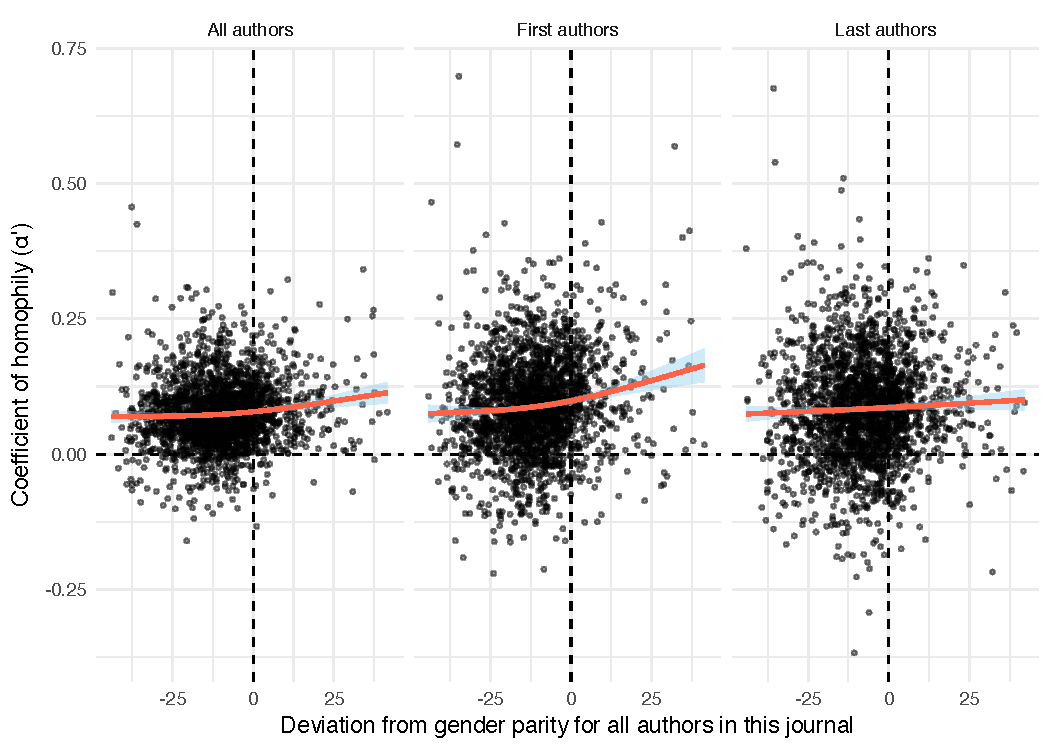
\includegraphics{../figures/figure3.pdf}
\caption{There is a weakly positive, non-linear relationship between the
gender ratio of authors publishing in a journal, and the coefficient of
homophily (\(\alpha'\)). Specifically, journals with 50\% women authors
or higher tended to have more same-sex coauthorships than did journals
with predominantly men authors. This relationship held whether
\(\alpha'\) was calculated for all authors, first authors only, or last
authors only. A negative value on the x-axis denotes an excess of men
authors, a positive value denotes an excess of women authors, and zero
denotes gender parity. The lines were fitted using generalised additive
models with the smoothing parameter \(k\) set to 3.
\label{alpha_gender_ratio}}
\end{figure}

\newpage

\begin{figure}
\centering
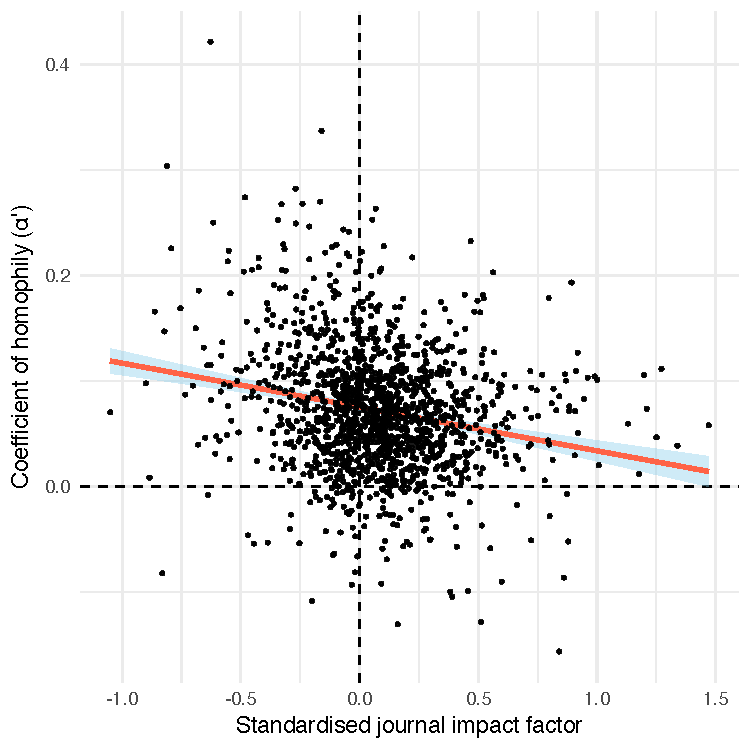
\includegraphics{../figures/figure4.pdf}
\caption{Journal impact factor (expressed relative to the average for
the discipline) is negatively correlated with \(\alpha'\). The
relationship is noisy (\(R^2\) = 0.043), but the results suggest that
journals with strong homophily tend to have lower impact factors than
journals with weak homophily in the same discipline.
\label{impact_factor}}
\end{figure}


\end{document}
